\section{TGA -- Temporal Graph Algebra}
\label{sec:algebra}

This section defines our proposed Temporal Graph Algebra, or \tga for
short.  Our goal is to enable a wide range of analyses useful to
potential users, with a focus on analysis over time, and motivated by
our examples and those we found in the literature.

The semantics of each operator is specified either by a translation
into a sequence of \tra operators~\cite{Dignos2012}, or by applying
navigational patterns~\cite{DBLP:journals/corr/AnglesABHRV16},
extended with time.  We assume that the model properties are
maintained by the temporal relational model, e.g., that if a \tra
operator is known to produce uncoalesced results, they are coalesced
in the final output, and that the integrity constraints from \te to
\tv are enforced.  We use the foreign key constraint enforcement
method that allows the operation and then modifies the output to
remove (or trim) tuples from \te for which a corresponding entry does
not exist in \tv.  For readability sake, we use a shorthand notation
and refer to $\tve.\tv$ as $\tv$ and to $\tve.\te$ as $\te$.

{\bf Trim.}  It is useful to focus analysis on a particular portion of
the overall \tg history.  The \insql{trim} operator computes a new
\tg, limited only to those nodes and edges that existed during the
specified period.

\begin{definition}[Trim]
\label{def:slice}
The trim operator, denoted \\$\slice{\bc}{\ttt}$, where
$\bc$ is a time interval and $\ttt$ is a \tg is defined as:

$\slice{\bc}{\ttt} = (TV', TE') ~|~$\\ $TV' = \pi_{v,T \text{ intersect } \bc,a}(\sigma^T_{p \text{ overlaps } \bc}(TV)) \land$ \\ $TE' = \pi_{e,v_1,v_2,T \text{ intersect } \bc,a}(\sigma^T_{p \text{ overlaps } \bc}(TE)$
\end{definition}

\begin{table}
\centering
\caption{$\slice{['15/5,'15/8)}{\ttt}$}
\vspace{-0.2cm}
\label{tab:slice}
\resizebox{\columnwidth}{!}{%
\begin{tabular}{| c | c | c | c | c |}
\hline
\multicolumn{5}{|l|}{$TV$} \\
\multicolumn{3}{|c}{\bfseries{\underline v}} & \multicolumn{1}{c}{\bfseries a} & \multicolumn{1}{c|}{\bfseries T} \\ \hline
\multicolumn{3}{|c|}{v1} & type=person,name=Alice,school=Drexel & ['15/5,'15/7) \\ \hline
\multicolumn{3}{|c|}{v2} & type=person,name=Bob,school=CMU & ['15/5,'15/8) \\ \hline
\multicolumn{3}{|c|}{v3} & type=person,name=Cathy,school=Drexel & ['15/5,'15/8) \\ \hline
\multicolumn{5}{|l|}{} \\
\multicolumn{5}{|l|}{$TE$} \\
\multicolumn{1}{|c}{\bfseries{\underline e}} & \multicolumn{1}{c}{\bfseries v1} & \multicolumn{1}{c}{\bfseries v2} & \multicolumn{1}{c}{\bfseries a} & \multicolumn{1}{c|}{\bfseries T} \\ \hline
e1 & v1 & v2 & type=co-author,cnt=3 & ['15/5,'15/6) \\ \hline
e2 & v2 & v3 & type=co-author,cnt=4 & ['15/7,'15/8) \\ \hline
\end{tabular}
}
\vspace{-0.2cm}
\end{table}

\vspace{-0.2cm}
\begin{example}
\label{ex:slice}
Consider the example \tg \ttt in Table~\ref{tab:tg}, which we use
throughout this section.  \insql{trim} with an input period
['15/5,'15/8) computes $\ttt'$ as depicted in Table~\ref{tab:slice}.
  Observe that tuple $x2$ is not present because it is wholly outside
  of the input period.  Observe also that the period of validity of
  tuple $x1$ has been modified to equal the intersection with the
  input period, i.e., it has been trimmed.
\end{example}

\insql{trim} is essentially a temporal selection over \tv and \te
relations to contain only those nodes and edges whose periods have a
non-empty intersection with $\bc$, with their periods trimmed to be
within $\bc$.  The selection can be performed over \tv and \te
relations in any order.

{\bf Map.}  To allow manipulation of node and edge attributes we
introduce {\bf vertex-map} and {\bf edge-map} operators.  Vertex-map
and edge-map apply user-defined map functions to attributes in the
same spirit as \insql{map} in functional languages and the relational
projection operator in \tra.

While the map functions are arbitrary user-specified functions, there
are some common cases.  Map may specify the set of properties to
project out or retain, it may aggregate (e.g., \insql{COUNT}) or
values of a collection property, or unnest a nested value in a
property.  In other words, mapping is on an entity-by-entity,
tuple-by-tuple basis.  The time period can be referenced in the
mapping function but cannot be changed, that is, the period of
validity remains unchanged.

\begin{definition}[vertex-map]
\label{def:vmap}
The vertex-map operator, denoted $\vmap{f_v,\ttt}$, where $f_v$ is a
user-defined mapping function, is defined as:

$\vmap{f_v,\ttt} = (TV', TE') ~|~ TV' = \{(v,a'|T)~|~ (v,a|T) \in \tv \land a'= f_v(v,a|T)\} \land TE' = TE$
\end{definition}

In other words, \insql{vertex-map} is essentially a temporal
projection over \tv that retains all attributes of \tv but changes the
nested attribute \insql{a}.  Because node periods are not modified, no
changes to \te are made to enforce referential integrity.  The $\tv'$
relation must be coalesced, which is done automatically by the model.

\begin{table}
\centering
\caption{$\vmap{\pi_{type,name},\ttt}$}
\vspace{-0.2cm}
\label{tab:vmap}
\resizebox{\columnwidth}{!}{%
\begin{tabular}{| c | c | c | c | c |}
\hline
\multicolumn{5}{|l|}{$TV$} \\
\multicolumn{3}{|c}{\bfseries{\underline v}} & \multicolumn{1}{c|}{\bfseries a} & \multicolumn{1}{c|}{\bfseries T} \\ \hline
\multicolumn{3}{|c|}{v1} & type=person,name=Alice & ['15/1,'15/7) \\ \hline
\multicolumn{3}{|c|}{v2} & type=person,name=Bob & ['15/2,'15/10) \\ \hline
\multicolumn{3}{|c|}{v3} & type=person,name=Cathy & ['15/1,'15/10) \\ \hline
\multicolumn{5}{|l|}{} \\
\multicolumn{5}{|l|}{$TE$} \\
\multicolumn{1}{|c}{\bfseries{\underline e}} & \multicolumn{1}{c}{\bfseries v1} & \multicolumn{1}{c}{\bfseries v2} & \multicolumn{1}{c|}{\bfseries a} & \multicolumn{1}{c|}{\bfseries T} \\ \hline
e1 & v1 & v2 & type=co-author,cnt=3 & ['15/2,'15/6) \\ \hline
e2 & v2 & v3 & type=co-author,cnt=4 & ['15/7,'15/10) \\ \hline
\end{tabular}
}
\vspace{-0.2cm}
\end{table}

\begin{example}
Consider again \tg \ttt in our running example from
Table~\ref{tab:tg}.  \insql{vertex-map} with a projection of the
\insql{type} and \insql{name} properties results in a new \tg,
depicted in Table~\ref{tab:vmap}.  Observe that tuples $x2$ and $x3$
generate only a single tuple over the combined time period due to
coalescing.
\end{example}

The \insql{edge-map} is defined similarly.

{\bf Subgraph.}  Temporal subgraph matching is a generalization of
subgraph matching for non-temporal graphs~\cite{Wood2012}.  Subgraph
returns a \tg matching the input navigational graph pattern that may
include temporal predicates.

To state this formally, we define a graph pattern to include time:

\begin{definition}[Temporal Navigational Graph Pattern]
\label{def:tngp}
A temporal navigational graph pattern (TNGP) is a graph $TNGP$, where
$V$ is extended with a set of node variables, $E$ is extended with a
set of edge variables and regular path expressions, and property names
and values are also extended with variables.  Any variable expression
may have a temporal predicate.

A match of TNGP in $G$ is restricted to be isomorphic, i.e., one
entity, whether node or edge, cannot match different variables.
When no temporal predicates are present in the TNGP, it is
  semantically evaluated as a regular navigational graph pattern over
  each snapshot of \ttt.
\end{definition}

We now define $\insql{subgraph}^T$ as follows:

\begin{definition}[Temporal subgraph]
\label{def:subv}
The temporal subgraph operator, denoted $\sub{P}{\ttt}$, where $q_v$
is a set of all nodes from node bindings of node variables and
constants in a temporal navigational graph pattern $P$, and $q_e$ is a
set of all edges from bindings of edge variables and constants in $P$,
is defined as:

$\sub{P}{\ttt} = (q_v(P,\ttt), q_e(P,\ttt),\Pi,\rho,\xi^T,\lambda^T_v,\lambda^T_e)$
\end{definition}

\begin{table}
\centering
\caption{$\insql{subgraph}^T$ with pattern $P_1$ returns a graph with no isolated nodes.}
\vspace{-0.2cm}
\label{tab:vsubgraph1}
\resizebox{\columnwidth}{!}{%
\begin{tabular}{| c | c | c | c | c |}
\hline
\multicolumn{5}{|l|}{$TV$} \\
\multicolumn{3}{|c}{\bfseries{\underline v}} & \multicolumn{1}{c}{\bfseries a} & \multicolumn{1}{c|}{\bfseries T} \\ \hline
\multicolumn{3}{|c|}{v1} & type=person,name=Alice,school=Drexel & ['15/2,'15/6) \\ \hline
\multicolumn{3}{|c|}{v2} & type=person,name=Bob & ['15/2,'15/5) \\ \hline
\multicolumn{3}{|c|}{v2} & type=person,name=Bob,school=CMU & ['15/5,'15/10) \\ \hline
\multicolumn{3}{|c|}{v3} & type=person,name=Cathy,school=Drexel & ['15/7,'15/10) \\ \hline
\multicolumn{5}{|l|}{} \\
\multicolumn{5}{|l|}{$TE$} \\
\multicolumn{1}{|c}{\bfseries{\underline e}} & \multicolumn{1}{c}{\bfseries v1} & \multicolumn{1}{c}{\bfseries v2} & \multicolumn{1}{c}{\bfseries a} & \multicolumn{1}{c|}{\bfseries T} \\ \hline
e1 & v1 & v2 & type=co-author,cnt=3 & ['15/2,'15/6) \\ \hline
e2 & v2 & v3 & type=co-author,cnt=4 & ['15/7,'15/10) \\ \hline
\end{tabular}
}
\vspace{-0.2cm}
\end{table}

\begin{figure}
\centering
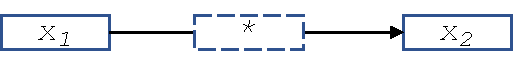
\includegraphics[width=2.5in]{figs/nonisolated.pdf}
\caption{Navigational graph pattern $P_1$, restricting to nonisolated nodes only.}
\vspace{-0.2cm}
\label{fig:nonisolated}
\vspace{-0.2cm}
\end{figure}

\vspace{-0.2cm}
\begin{example}
Consider \tg \ttt from our running example (Table~\ref{tab:tg}).
Let's say that we are only interested in non-isolated nodes, i.e.,
only those that have a non-zero degree.  Pattern $P_1$, shown in
Figure~\ref{fig:nonisolated}, yields new \tg \ttt' depicted in
Table~\ref{tab:vsubgraph1}.  Observe that while the number of node
tuples in the output is the same as in the input, their periods are
smaller to only include times when edges are present.  For instance,
$x1$ period has been reduced from ['15/1,'15/7) to ['15/2,'15/6),
    since no edge connected to $v1$ exists in either ['15/1,'15/2)
      or ['15/6,'15/7).
\end{example}

{\bf Aggregation.}  Temporal aggregation is a generalization of the
graph aggregation operation~\cite{Wood2012} to include temporal
predicates and operate over temporal data.  It computes the value of a
new node property based on information available at the node itself,
at the edges associated with the node, and at its neighbors.
Aggregation can be used to compute simple properties such as in-degree
of a node, or more complex ones such as the set of countries that the
friends of $v$ visited in the past year.

\begin{definition}[Aggregation]
\label{def:tgagg}
Temporal graph aggregation $\insql{agg}^T(P,G)$, where $q_v$ is a set
of all nodes from node bindings of node variables with aggregation
functions in a TNGP (Definition~\ref{def:tngp}) $P$ is defined as:

$\insql{agg}^T(P,G) = (TV',TE') ~|~ TV' = TV \cup^T q_v(P,\ttt) \land TE' = TE$
\end{definition}

Aggregation can be used to compute the lengths of {\em journeys}.  A
journey is transitive closure on the graph conditional on the time
property of the edges -- two nodes are connected by a new edge if
there is a non-decreasing time path between
them~\cite{Casteigts2011,Ferreira2004}.

\begin{example}
Consider \tg \ttt in our running example.  We can compute the longest
journey from each node in \ttt using aggregation.  The longest journey
from node $v1$ is of length 2 through node $v2$ to node $v3$, since
edge tuple $y2$ starts later than tuple $y1$.  However, node $v1$ is
unreachable from node $v3$ even if we reverse the edge direction because
that requires traveling back in time.
\end{example}

{\bf Node creation.}  The node creation operator enables the user to
analyze an evolving graph at different levels of granularity.  This
operator comes in two variants --- based on node attributes or based
on temporal window.

Attribute-based node creation is a temporal generalization of the
graph node creation operation~\cite{Wood2012}.  Node creation adds new
nodes that represent a matching input pattern.  Attribute-based node
creation takes in a TNGP extended with Skolem functions, but is
otherwise the same as the nontemporal one.

\begin{definition}[Attribute-based node creation]
\label{def:nodecra}
Attribute-based node creation, denoted $\insql{node}^T_a(P,\ttt)$
where $q_v$ is a set of nodes in TNGP $P$ with an expression containing a
Skolem function, and $q_e$ is a set of edges in $P$ with an expression
containing a Skolem function, is defined as:

$\insql{node}^T_a(P,\ttt) = (TV',TE') ~|~ TV' = q_v(P,\ttt) \land TE' = q_e(P,\ttt)$
\end{definition}

Intuitively, like in the non-temporal version, the nodes are computed
by applying the pattern.  Every new node is assigned an identity by a
Skolem function.  Each new node is connected to the pattern from which
it originated with new edges, the identity of which is also assigned
by a Skolem function.

Attribute-based node creation allows the user to, for instance,
generate a \tg in which nodes correspond to disjoint groups of nodes
in the input that agree on the values of all grouping attributes.  It
can also be used with more complex patterns, such as to generate a new
node for each connected component and assign it a size property.

\begin{figure}
\centering
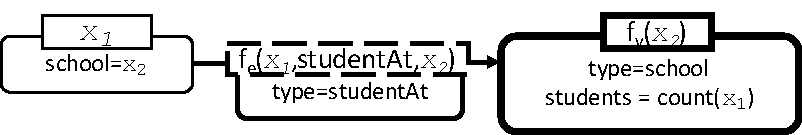
\includegraphics[width=3in]{figs/schoolncr.pdf}
\caption{TNGP to create nodes for each value of school property.}
\vspace{-0.2cm}
\label{fig:schoolncr}
\vspace{-0.2cm}
\end{figure}

\begin{table}
\centering
\caption{Attribute-based node creation based on property \insql{school}.}
\vspace{-0.2cm}
\label{tab:nodecra1}
\resizebox{\columnwidth}{!}{%
\begin{tabular}{| c | c | c | c | c |}
\hline
\multicolumn{5}{|l|}{$TV$} \\
\multicolumn{3}{|c}{\bfseries{\underline v}} & \multicolumn{1}{c}{\bfseries a} & \multicolumn{1}{c|}{\bfseries T} \\ \hline
\multicolumn{3}{|c|}{v1} & type=person,name=Alice,school=Drexel & ['15/1,'15/7) \\ \hline
\multicolumn{3}{|c|}{v2} & type=person,name=Bob & ['15/2,'15/5) \\ \hline
\multicolumn{3}{|c|}{v2} & type=person,name=Bob,school=CMU & ['15/5,'15/10) \\ \hline
\multicolumn{3}{|c|}{v3} & type=person,name=Cathy,school=Drexel & ['15/1,'15/10) \\ \hline
\multicolumn{3}{|c|}{Drexel} & type=school,students=2 & ['15/1,'15/7) \\ \hline
\multicolumn{3}{|c|}{Drexel} & type=school,students=1 & ['15/7,'15/10) \\ \hline
\multicolumn{3}{|c|}{CMU} & type=school,students=1 & ['15/5,'15/10) \\ \hline
\multicolumn{5}{|l|}{} \\
\multicolumn{5}{|l|}{$TE$} \\
\multicolumn{1}{|c}{\bfseries{\underline e}} & \multicolumn{1}{c}{\bfseries v1} & \multicolumn{1}{c}{\bfseries v2} & \multicolumn{1}{c}{\bfseries a} & \multicolumn{1}{c|}{\bfseries T} \\ \hline
e1 & v1 & v2 & type=co-author,cnt=3 & ['15/2,'15/6) \\ \hline
e2 & v2 & v3 & type=co-author,cnt=4 & ['15/7,'15/10) \\ \hline
e3 & v1 & Drexel & type=studentAt & ['15/1,'15/7) \\ \hline
e4 & v3 & Drexel & type=studentAt & ['15/1,'15/10) \\ \hline
e5 & v2 & CMU & type=studentAt & ['15/5,'15,10) \\ \hline
\end{tabular}
}
\vspace{-0.2cm}
\end{table}

\begin{example}
Consider our running example \tg \ttt (Table~\ref{tab:tg}).  We can
create new summary nodes to represent each school based on the
\insql{school} property of the nodes using the pattern in
Figure~\ref{fig:schoolncr}.  The result is shown in
Table~\ref{tab:nodecra1}, with two new nodes \insql{Drexel} and
\insql{CMU} and \insql{studentAt} edges connecting to these nodes.
The TNGP can specify aggregation functions to compute properties of
the new nodes based on the input pattern and here \insql{count} is
used to generate the \insql{students} property.
\end{example}

It is interesting and insightful to analyze an evolving graph at
different levels of temporal granularity.  For example, the user may
want to redefine temporal resolution and look at the graph at that
scale, irrespective of whether this resolution happens to be finer or
coarse than the natural evolution rate of the graph.  For this, we
introduce a window-based node creation operator that is similar to the
{\em moving window temporal aggregation} in temporal relational
algebra.  Our approach is inspired by stream aggregation work
of~\cite{Li2005}, adopted to graphs, and by generalized quantifiers
of~\cite{Hsu1995}.

Window-based node creation modifies tuple periods based on consecutive
temporal windows from the window specification, such as \insql{2
  months} or \insql{10 years}.

It is useful to be able to quantify required node/edge duration in
order to consider it valid.  We use {\em quantifiers} for this
purpose.  Node and edge quantifiers $r_v$ and $r_e$ are of the form \{
\insql{all} | \insql{most} | \insql{at least} $n$ | \insql{exists} \},
where $n$ is a decimal representing the percentage of the time during
which a node or an edge existed, relative to the duration of the
window.  Quantifiers are useful for observing different kinds of
temporal evolution, e.g., to observe only strong connections over a
volatile evolving graph, we may want to only include nodes that span
the entire window ($r_v=\insql{all}$), and edges that span a large
portion of the window ($r_e=\insql{most}$).

Window specification is of the form $n~\{unit|\insql{changes}\}$,
where $n$ is an integer, and $unit$ is a time unit, e.g., \insql{10
  min}, \insql{3 years}, or any multiple of the usual time units.
When the window specification is in the form $n~\insql{changes}$, it
defines the window by the number of changes that occurred in \ttt
(affecting any of its constituent relations). Window boundaries are
defined left-to-right, i.e., from least to most recent.

Window specification generates a temporal relation $W$ with the schema
$(N|T)$, where each tuple associates a window number with its
duration.

Putting it all together:

\begin{definition}[Window-based node creation]
\label{def:nodecrw}
The window-based node creation operator, denoted
$\insql{node}^T_w(w,r_v,r_e,f_{v_1}(k_1)\varlist f_{v_n}(k_n),f_{e_1}(l_1)\varlist f_{e_m}(l_m),\ttt)$,\\
where $w$ is the window specification, $W$ is the relation generated
by $w$ consisting of periods defined by the specification, $r_v$ and
$r_e$ are node and edge quantifiers, and each $f_{v_j}(k_j)$
($f_{e_j}(l_j)$) specifies an aggregation function $f_{v_j}$
(resp. $f_{e_j}$) to be applied to a node property $k_j$ (resp. edge
property $l_j$) is defined as:

%\begin{align}
$\insql{node}^T_w(w,r_v,r_e,f_{v_1}(k_1)\varlist f_{v_n}(k_n),f_{e_1}(l_1)\varlist f_{e_m}(l_m),\ttt) = (TV', TE') ~|~ $\\$TV' = \nu_{k_1\varlist k_n,a}(\sigma^T_{r_v}(\resolve{f_{v_1}(k_1)\varlist f_{v_n}(k_n)}{\break\mu^T_a(\pi^T_{v,a}(TV \times^T W))})) ~\land$\\
$TE' = \nu_{l_1\varlist l_m,a}(\sigma^T_{r_e}(\resolve{f_{e_1}(l_1)\varlist f_{e_m}(l_m)}{\mu_a(\break\pi^T_{e,v1,v2,a}(TE \times^T W))}))$
%\end{align}
\end{definition}

Essentially, we compute a cross product of each node and edge to every
window it overlaps, project out the dummy window number, unnest
($\mu$), apply the resolve primitive for cases
where more than one identity-equivalent tuple is in the same window,
select only those that meet the quantification, and finally re-nest
($\nu$).  It does not matter in which order
computation is applied, i.e., either \tv or \te can be computed first,
as long as the foreign key constraint is enforced in the final result.

For the purposes of this operator we expand the list of supported
aggregation functions to include temporal \insql{first}
($min(t_1.s,t_2.s)$) and \insql{last} ($max(t_1.s,t_2.s)$).

Our window specification by change is similar to slide-by-row window
in stream aggregation~\cite{Li2005}.  Note that, because \tg algebra
is compositional, we do not support node creation with overlapping
windows, because it does not produce a valid \tg.  To see why this is
so, consider applying a sliding window of 3 months range with 1 month
slide to graph \insql{T} in our running example \tg \ttt.  We would
produce the following tuples for $v_1$: $(v_1, ['15/1, '15/4), a_1)$,
  $(v_1, ['15/2, '15/5), a_2)$, $(v_1, ['15/3, '15/6))$, and so on, which
      clearly violates the temporally coalesced requirement in
      definition~\ref{def:tg2}.

\begin{table}
\centering
\caption{$\insql{node}^T_w(r_v=\insql{always},r_e=\insql{exists},f_{v_1}=\insql{first(name)},f_{v_2}=\insql{first(school)},\ttt)$}
\vspace{-0.2cm}
\label{tab:nodecrw2}
\resizebox{\columnwidth}{!}{%
\begin{tabular}{| c | c | c | c | c |}
\hline
\multicolumn{5}{|l|}{$W$} \\
\multicolumn{4}{|c}{\bfseries{\underline N}} & \multicolumn{1}{c|}{\bfseries T} \\ \hline
\multicolumn{4}{|c}{1} & ['15/1,'15/6) \\ \hline
\multicolumn{4}{|c}{2} & ['15/6,'1510) \\ \hline
\multicolumn{5}{|l|}{} \\
\multicolumn{5}{|l|}{$TV$} \\
\multicolumn{3}{|c}{\bfseries{\underline v}} & \multicolumn{1}{c}{\bfseries a} & \multicolumn{1}{c|}{\bfseries T} \\ \hline
\multicolumn{3}{|c|}{v1} & type=person,name=Alice,school=Drexel & ['15/1,'15/6) \\ \hline
\multicolumn{3}{|c|}{v2} & type=person,name=Bob,school=CMU & ['15/5,'15/10) \\ \hline
\multicolumn{3}{|c|}{v3} & type=person,name=Cathy,school=Drexel & ['15/1,'15/10) \\ \hline
\multicolumn{5}{|l|}{} \\
\multicolumn{5}{|l|}{$TE$} \\
\multicolumn{1}{|c}{\bfseries{\underline e}} & \multicolumn{1}{c}{\bfseries v1} & \multicolumn{1}{c}{\bfseries v2} & \multicolumn{1}{c}{\bfseries a} & \multicolumn{1}{c|}{\bfseries T} \\ \hline
e1 & v1 & v2 & type=co-author,cnt=3 & ['15/5,'15/6) \\ \hline
e2 & v2 & v3 & type=co-author,cnt=4 & ['15/6,'15/10) \\ \hline
\end{tabular}
}
\vspace{-0.2cm}
\end{table}

\begin{example}
\label{ex:nodecrw2}
Table~\ref{tab:nodecrw2} illustrates window-based node creation by
change ($w=3~\textsf{changes}$) with \insql{all} quantifier for
nodes and \insql{exists} for edges, and \insql{first} aggregation
function for node and edge properties.  \eat{The windows computed
  with this specification are ['15/1,'15/6) and
    ['15/6,'15/10). }$v_2$ is present in the result starting at
    $'15/5$ because it did not exist for the entirety of the first
    window.  Edge id $e1$ is reduced in duration because before '15/5
    $v2$ does not exist and after '15/6 $v1$ does not exist.  On the
    other hand edge id $e2$ is extended in duration to cover the whole
    second window as both of its end points exist and it existed at
    some point during the window in the input.
\end{example}

{\bf Set-based operators.}  We support temporal versions of the three binary set operators
intersection ($\cap^{TG}$), union ($\cup^{TG}$), and difference
($\setminus^{TG}$).  The union operator produces a \tg that contains
nodes and edges that exist in either $\ttt_1$ or $\ttt_2$.

There is a graph-specific difference between \tra union and \tga union
related to identity, namely, there is no guarantee that a node or an
edge with the same identity and at the same time instant has the same
property set in both input graphs.  Previously published work either
avoided this problem by not using the property model (as long as ids
match there is no issue) or side-stepped it by requiring that both
input graphs are drawn from the same underlying graph
\eat{~\cite{Amer-Yahia2009}}.  We aim to provide a more general operation
without this restriction.  To this end we require aggregation
functions as additional input to $\cup^{TG}$ to resolve
identity-equivalent tuples with overlapping periods.

\begin{definition}[Union]
\label{def:uniontg}
\tg union operator, denoted $\cup^{TG}_{f_{v1}(k_1),\ldots,f_{vn}(k_n),f_{e1}(l_1),\ldots,f_{em}(l_m)}$,
where each $f_{vj}(k_j)$ (resp. $f_{ej}(l_j)$) specifies an aggregation
function $f_{vj}$ (resp. $f_{ej}$) to be applied to a node property
$k_j$ (resp. edge property $l_j$) is defined as:

$\ttt_1 \cup^{TG}_{f_{v1}(k_1),\ldots,f_{vn}(k_n),f_{e1}(l_1),\ldots,f_{em}(l_m)} \ttt_2 = (TV', TE') ~|~$\\$TV' = \resolve{f_{v1},\ldots,f_{vn}}{TV_1 \cup^T TV_2} \land$\\$TE' = \resolve{f_{e1},\ldots,f_{em}}{TE_1 \cup^T TE_2}$
\end{definition}

We use the \tra's $\cup^T$ operator on both constituent relations of
\ttt, followed by applying the resolve primitive to coalesce
identity-equivalent tuples.  With this approach nodes (resp. edges)
can have different property sets while still resulting in a valid
output \tg.  Note, however, that it is still necessary for the node
(resp. edge) identifiers of the two graphs to be from the same
universe.

For the purposes of binary operators we expand the set of aggregation
functions to include \insql{left}, which gives precedence to the value
of the property from the left operand, and \insql{right}, which does
the opposite.  These functions are useful if it is known that one of
the two input \tgs contains the ground truth.

The \tg intersection operator produces a \tg of nodes and edges that
exist in both $\ttt_1$ and $\ttt_2$ and is defined in a similar fashion
as the union operator:

\begin{definition}[Intersection]
\label{def:intertg}
%\hfill \break
\tg intersection operator, denoted
$\cap^{TG}_{f_{v1}(k_1),\ldots,f_{vn}(k_n),f_{e1}(l_1),\ldots,f_{em}(l_m)}$,
where each $f_{vj}(k_j)$ ($f_{ej}(l_j)$) specifies an aggregation
function $f_{vj}$ (resp. $f_{ej}$) to be applied to a node property
$k_j$ (resp. edge property $l_j$) is defined as:

$\ttt_1 \cap^{TG}_{f_{v1}(k_1),\ldots,f_{vn}(k_n),f_{e1}(l_1),\ldots,f_{em}(l_m)} \ttt_2 = (TV', TE') ~|~ $\\$TV' = \resolve{f_{v1},\ldots,f_{vn}}{TV_1 \Join^T_{v} TV_2} \land $\\$TE' = \resolve{f_{e1},\ldots,f_{em}}{TE_1 \Join^T_{e} TE_2}$
\end{definition}

Instead of using the \tra set intersection operator we must use an
inner join to allow for tuples that identity-equivalent but have
different property sets.  If we use set intersection,
identity-equivalent tuples that are not value-equivalent would be
eliminated.  We apply the resolve primitive in the usual manner.
There is no dependence between computation of \tv and \te -- it can be
done in any order or in parallel.

The difference operator produces nodes and edges that exist in
$\ttt_1$ but not in $\ttt_2$.  It does not require aggregation
functions for resolution but is otherwise defined in a similar manner:

\begin{definition}[Difference]
\label{def:difftg}
\tg difference operator, denoted
$\setminus^{TG}$ is defined as:

$\ttt_1 \setminus^{TG} \ttt_2 = (TV', TE') ~|~ $\\$TV' = \pi^T_{TV_1.v,TV_1.a}(\sigma^T_{TV_2.a is NULL}(TV_1 \leftouterjoin^T_{v} TV_2)) \land $\\$TE' = \pi^T_{TE_1.e,TE_1.v1,TE_1.v2,TE_1.a}(\sigma^T_{TE_2.a is NULL}(TE_1 \leftouterjoin^T_{e} TE_2))$
\end{definition}

Since we operate based on node (resp. edge) identity rather than tuple
equivalence, instead of the \tra's difference operator we use a left
outer join, select only those tuples that exist in $\ttt_1$ but not in
$\ttt_2$ using the $not NULL$ predicate, and then project out the
extra columns.

{\bf Edge creation.}  Edge creation is a binary operator and is a
temporal generalization of the various non-temporal graph products.
The reason we call it {\bf edge creation} is because the edges
produced in the output may not exist in either of the two input
graphs.

The nodes in the two input graphs are combined, while the edges are
computed with a temporal navigational graph pattern extended with
namespaces.

\begin{definition}
\label{def:edgecr}
The edge creation operator $\insql{edge}^T_{P}(\ttt_1,\ttt_2)$, where
$q_e$ is a set of edges with an expression containing a Skolem
function in a TNGP $P$ over $\ttt_1$ and $\ttt_2$ extended with
namespaces, and each $f_{vj}(k_j)$ specifies an aggregation function
$f_{vj}$ to be applied to a node property $k_j$, is defined as:

$\textsf{edge}^T_{P,f_{v1}(k_1),\ldots,f_{vn}(k_n)}(\ttt_1,\ttt_2) = (TV',TE') ~|~ \break TV' = \resolve{f_{v1},\ldots,f_{vn}}{TV_1 \cup^T TV_2} \land TE' = q_e(P,\ttt_1,\ttt_2)$
\end{definition}

Similar to node creation, a Skolem function is required to assign
identity to new edges.  The nodes are generated exactly as in the
temporal union $\cup^{TG}$.  Intuitively, edge creation returns a
new \tg from nodes of $\ttt_1$ and $\ttt_2$, connected by edges
determined by the input pattern.

Edge creation has several important applications.  It can be used to
transpose \tg edges or compute friend-of-friend edges, passing in the
same \tg as both arguments.  Since $P$ can be recursive and include
predicates over the timestamps, $\insql{edge}^T$ can create new edges
representing journeys.  Recall that a journey is a path in the
evolving graph with non-decreasing time edges.  By adding a temporal
condition to $P$, we can obtain journeys similar to time-concurrent
paths.



